\begin{figure}[h]
  \begin{center}

    %\tikzstyle{c} = [draw=black,minimum width=1.5cm,minimum height=1cm]
    %\tikzstyle{a} = [draw, -latex',thick]

    %\begin{tikzpicture}
  %
  %     \node[c] (C) at (-4, -2) {
  %       \textbf{Corpus} of documents
  %     };
  %
  %     \node[c] (S) at (-4, 2) {
  %       \textbf{Spotter}
  %     };
  %
  %     \node[c] (H) at (-3, 0) {
  %       \textbf{Harvest}
  %     };
  %
  %     \node[c] (SA) at (1, 0) {
  %       \textbf{Search Algorithm}
  %     };
  %
  %     \node[c] (R) at (2, 2) {
  %       \textbf{Result Page}
  %     };
  %
  %     \node[c] (Q) at (2, -2) {
  %       \textbf{Query Input Page}
  %     };
  %
  %     \draw [a] Q.west -| SA.east;
  %
  %   \end{tikzpicture}
  \usetikzlibrary{fit,arrows,calc,positioning}
  \tikzstyle{comp} = [rectangle, draw, node distance=3cm, text width=6em, text centered, rounded corners, minimum height=4em, thick]
  \tikzstyle{compB} = [comp, fill=blue!20]
  \tikzstyle{compF} = [comp, fill=yellow!20]
  \tikzstyle{inter} = [draw, -latex',thick]

  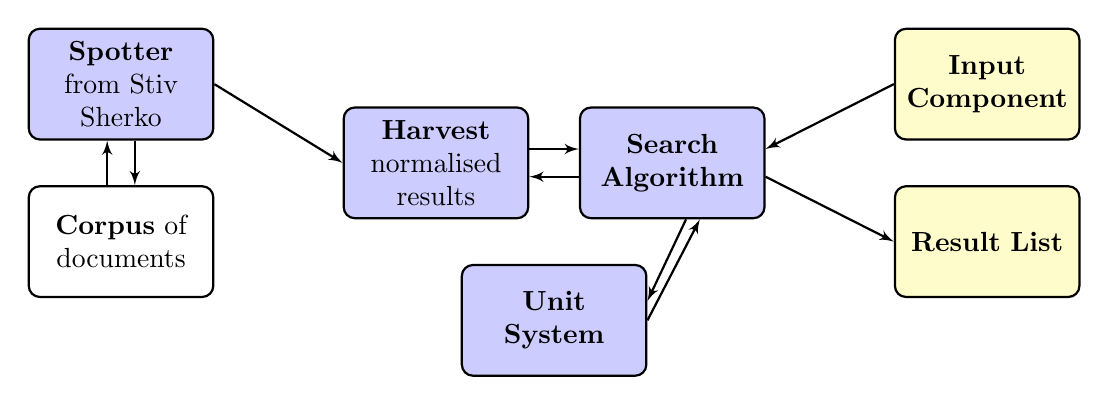
\begin{tikzpicture}[auto]
      \node [comp] (Q) at (-4, -1) {
        \textbf{Corpus} of documents
      };

      \node [compB] (S) at (-4, 1) {
        \textbf{Spotter} from Stiv Sherko
      };

      \draw [inter] ([xshift=-5pt] Q.north) -- ([xshift=-5pt] S.south);
      \draw [inter] ([xshift=5pt] S.south) -- ([xshift=5pt] Q.north);

      \node [compB] (H) at (0, 0) {
        \textbf{Harvest} normalised results
      };

      \draw [inter] (S.east) -- (H.west);

      \node [compB] (SA) at (3, 0) {
        \textbf{Search Algorithm}
      };

      \draw [inter] ([yshift=5pt] H.east) -- ([yshift=5pt] SA.west);
      \draw [inter] ([yshift=-5pt] SA.west) -- ([yshift=-5pt] H.east);

      \node [compF] (R) at (7, -1) {
        \textbf{Result List}
      };

      \draw [inter] ([yshift=-5pt] SA.east) -- (R.west);

      \node [compF] (Q) at (7, 1) {
        \textbf{Input Component}
      };

      \draw [inter] (Q.west) -- ([yshift=5pt] SA.east);

      \node [compB] (US) at (1.5, -2) {
        \textbf{Unit System}
      };

      \draw [inter] (US.east) -- ([xshift=10pt] SA.south);
      \draw [inter] ([xshift=5pt] SA.south) -- ([yshift=7pt] US.east);

  \end{tikzpicture}

  \end{center}

  \caption{Basic Architecture Of The System. Components Of The Backend Are Drawn In Blue, Components Of The Frontend In Yellow. }
  \label{fig:system}
\end{figure}
